\section{Ziel}
Das Ziel dieses Versuchs ist es die Suszeptibilität paramagnetischer Substanzen mit
zwei unterschiedlichen Methoden sowie theoretisch zu bestimmen.
Diese Substanzen werden Seltene-Erd-Verbindungen genannt. 

\section{Theorie}
\label{sec:Theorie}

%Der Drehimpuls J und der Landé-Faktor $g_J$ müssen bestimmt werden, um die Suszeptibilität 
%bestimmen zu können. Für ein $Pr^{3+}$-Ion ergibt sich $g_J= 0.8$.

\subsection{Theoretische Grundlagen}
Im Folgenden werden zunächst für den Versuch relevante Dinge erklärt.

\subsubsection{Magnetisierung}
Die magnetischen Flussdichte $\vec{B}$ ändert sich in Materie um die Magnetisierung $\vec{M}$-
Diese entsteht durch atomare magnetische Momente. %innerhalb einer Probe. 
%Sie ergibt sich als Produkt des mittleren magnetischen Moments \bar{\vec{\mu}}, der magnetischen Permeabilität und der Anzahl $N$ der Momente pro Volumeneinheit. 
Sie ist abhängig von der magnetischen Feldstärke $\vec{H}$:
\begin{equation*}
    \vec{M} = \mu_0 \chi \vec{H}.
    \label{eqn:magnetisierung}
\end{equation*}
Dabei ist $\chi$ die Suszeptibilität, welche von der magnetischen Feldstärke $H$ und 
der Temperatur $T$ abhängt. 

\subsubsection{Paramagnetismus}
%Da es sich bei der Magnetisierung um Paramagnetismus handelt, ergibt sich daraus, warum die Suszeptibilität temperaturabhängig ist. 
Paramagnetismus tritt bei Atomen, die einen Drehimpuls besitzen, auf. 
Er entsteht durch die Orientierung der magnetischen Momente zu einem äußeren Feld. 
Die Ausrichtung ist durch thermische Bewegung gestört, weshalb der Paramagnetismus 
temperaturabhängig ist. 

\subsubsection{Drehimpuls}
Der Gesamtdrehimpuls $\vec{J}$ eines Atoms setzt sich hier nur aus dem Gesamtbahndrehimpuls und dem Gesamtspin 
zusammen. Die Gesamtdrehimpulsquantenzahl ist gegeben durch
\begin{equation*}
    |\vec{J}| = |\vec{L}| + |\vec{S}|.
\end{equation*}
Für die Summanden gilt
\begin{align*}
   |\vec{L}| &= \sqrt{L(L+1)} \hbar \\
   |\vec{S}| &= \sqrt{S(S+1)} \hbar,
\end{align*}
wobei $L$ die Bahndrehimpulsquantenzahl und $S$ die Spinquantenzahl ist.

\subsubsection{Seltene-Erd-Verbindungen}
Verbindungen, die Ionen Seltener Erden enthalten, sind stark paramagnetisch. 
Die Elektronenhülle dieser Atome muss also große Drehimpulse besitzen. 
Diese werden von inneren Elektronen erzeugt, weil der Effekt auch bei Ionen zu erkennen ist. 
Der Paramagnetismus Seltener Erden entsteht durch die 4f-Elektronen. %, die vom Cer an in die Elektronenhülle eingebaut werden. 


\subsubsection{Hundsche Regeln}
Die Hundschen Regeln definieren die Anordnung der Elektronen
in der unabgeschlossenen 4f-Schale
und den Gesamtdrehimpuls $\vec{J}$.
\begin{itemize}
\item Die Spins $\vec{s}_\text{i}$ summieren sich zum maximalen Gesamtspin, der nach dem 
Pauli-Prinzip möglich ist.
\item Der maximale Drehimpuls ist die Summe der Bahndrehimpulse $\vec{l}_\text{i}$. Er 
muss mit dem Pauli-Prinzip und der ersten Regel verträglich sein. 
\item Es gilt $\vec{J}= \vec{L} - \vec{S}$, wenn die Schale weniger als halb voll und 
$\vec{J}= \vec{L} + \vec{S}$, wenn die Schale mehr als halb voll ist.
\end{itemize}

\subsubsection{Unterdrückung von Störspannungen mittels Selektivverstärker}
Um die Brückenspannung zu messen muss die Störspannung herausgefiltert werden. 
Dazu wird ein Selektivverstärker verwendet, weil
die Brückenspannung eine monofrequente Spannung ist. Die Druchlassfrequenz $\nu_0$ des 
Selektivverstärkers wird auf die Signalfrequenz gestellt. 
Frequenzen, die nah an der Frequenz $\nu_0$ liegen, werden nicht herausgefiltert.
Eine Filterkurve eines Selektivverstärkers ist in Abb. \ref{abb:filterkurve} zu sehen.

\noindent Die Fitkurve des Selektivverstärkers lässt sich als Cauchy-Verteilung betrachten. Damit hat die Kurve die Form 
\begin{equation}
    f(x) = a \frac{1}{\pi} \frac{s}{s^2 + (x-t)^2}.
    \label{cauchyverteilung}
\end{equation}

\noindent Die Güte $Q$ des Selektivverstärkers ist durch
\begin{equation}
    Q = \frac{\nu_0}{\nu_\text{+} - \nu_\text{-}}
    \label{eqn:guete}
\end{equation}
definiert.

\begin{figure}
    \centering
    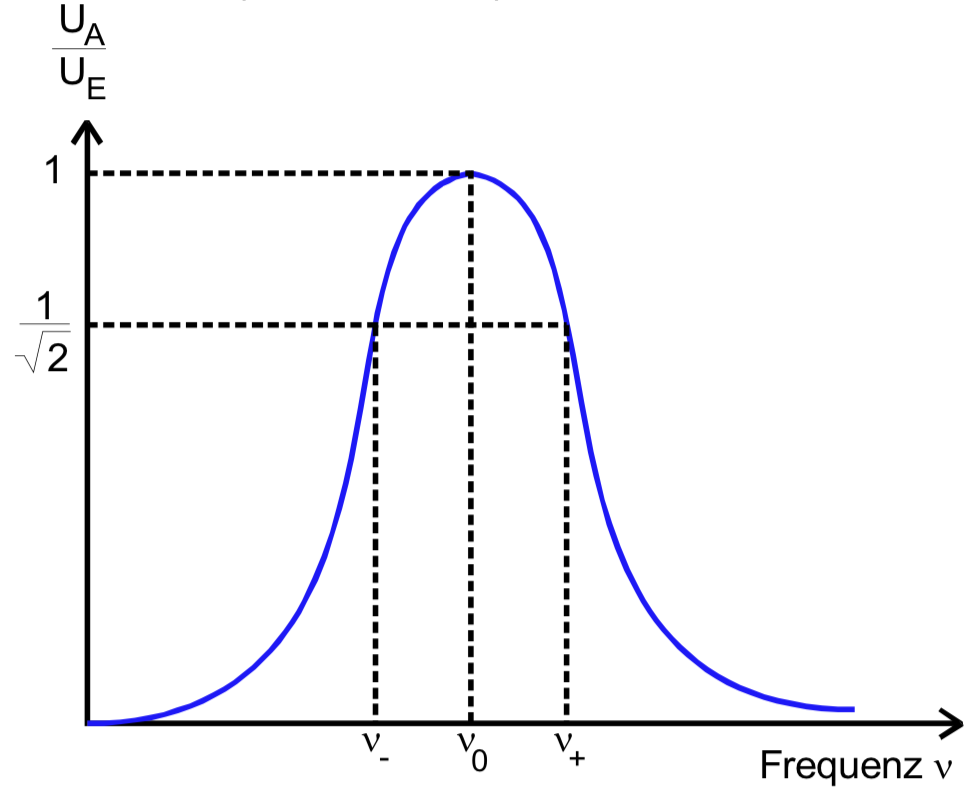
\includegraphics[width=10cm, height=8cm]{build/filterkurve.png}
    \caption{Filterkurve eines Selektivverstärkers. Die Frequenz ist gegen das
    Verhältnis von Ausggangs- und Eingangsspannung aufgetragen. Es sind die
    Druchlassfrequenz $\nu_0$ sowie die Frequenzen, bei denen das Verhältnis der
    Spannungen $\frac{1}{\sqrt{2}}$ beträgt, eingetragen. \cite{V606}}
    \label{abb:filterkurve}
\end{figure}


\subsection{Berechnung der theoretischen Suszeptibilität}
Die Suszeptibilität kann durch 
\begin{equation}
    \chi = \frac{\mu_0 \, \mu_\text{B}^2 \, g_\text{J}^2 \, N \, J \, (J+1)}{3 \, k_\text{B} \, T}
    \label{eqn:chitheo}
\end{equation}
bestimmt werden.
Dabei ist $k_\text{B}$ die Boltzmann-Konstante, $T$ die Temperatur und $N$ die Anzahl der 
Momente pro Volumeneinheit.
$N$ berechnet sich mit 
\begin{equation}
    N = 2 \, n_A \, \frac{\rho}{M},
    \label{N}
\end{equation}
wobei $n_A$ die Avogadrokonstante, $\rho$ die Dichte des Stoffs und $M$ die Molmasse des Stoffs ist. 

\noindent Außerden ist
\begin{equation*}
    \mu_\text{B} = \frac{1}{2} \frac{e_0}{m_0} \hbar 
\end{equation*}
das Bohrsche Magneton mit der Ladung $e_0$ und der Masse $m_0$ des Elektrons und dem Plankschen 
Wirkungsquantum $\hbar$. Der sogenannte Landé-Faktor ist als 
\begin{equation*}
    g_\text{J}= \frac{3 J(J+1) + (S(S+1) - L(L+1))}{2J(J+1)}
\end{equation*}
definiert. Hier ist $J$ wieder die Gesamtdrehimpulsquantenzahl, $S$ die Spinquantenzahl und $L$ 
die Bahndrehimpulsquantenzahl.


\subsection{Berechnung der Suszeptibilität mittels Brückenspannung}
Die Suszeptibilität kann mittels Induktivitätsmessung einer Spule
bestimmt werden.

\noindent Die Induktivität einer Zylinderspule ist durch
\begin{equation*}
    L = \mu_0 \frac{n^2 \, F}{l}
\end{equation*}
gegeben.
Dabei ist $n$ die Windungszahl, $F$ die Querschnittsfläche und $l$ die Länge der Spule.
Die Induktivität einer Spule, die vollständig mit Materie gefüllt ist,
unterscheidet sich um den Faktor $\mu_\text{r}$.
Der Querschnitt $Q$ einer Probe im Inneren der Spule ist kleiner als der Querschnitt 
der Spule.
Damit ändert sich die Induktivität insgesamt zu 
\begin{equation*}
    L_\text{M}= \mu_0 \, \frac{n^2 \, F}{l} + \chi \, \mu_0 \, \frac{n^2 \, Q}{l}.
    \label{eqn:induktivität}
\end{equation*}
Die Änderung der Induktivität ist also %Ist das darüber wichtig?
\begin{equation*}
    \Delta L = \mu_0 \, \chi \, Q \, \frac{n^2}{l}.
\end{equation*}

\noindent Die Suszeptibilität kann mittels des Verhältnisses der Brückenspannung $U_\text{Br}$
und der Speisespannung $U_\text{Sp}$ bestimmt werden
\begin{equation}
    \chi = 4 \, \frac{F}{Q} \, \frac{U_\text{Br}}{U_\text{Sp}}.
    \label{eqn:chiexp1}
\end{equation}
Dabei wird der Querschnitt der Probe folgendermaßen definiert
\begin{equation*}
    Q = \frac{M}{d \, \rho},
\end{equation*}
wobei $M$ die Masse, $d$ die Länge und $\rho$ die Dichte der Probe ist.


\subsection{Berechnung der Suszeptibilität mittels Abgleichbedingung} %Widerstandsverhältnis statt Abgleichbedingung?
%Die Abgleichbedingung, die dabei zu erfüllen ist, führt dazu, dass der Widerstand $R_3$ und der Widerstand $R_4$ annähernd gleich sein müssen. 
Nach dem Einführen einer Probe in eine Spule erhöht sich die Brückenspannung.
Das Verhältnis aus dem Wert $\Delta R$, um den der Widerstand $R_3$ korrigiert werden
muss, und diesem Widerstand $R_3$ kann genutzt werden, um die Suszeptibilität zu 
bestimmen:
\begin{equation}
    \chi = 2 \, \frac{\Delta R}{R_3} \, \frac{F}{Q}.
    \label{eqn:chiexp2}
\end{equation}